\documentclass{article}
\usepackage[utf8]{inputenc}
\usepackage[T1]{fontenc}
\usepackage{ngerman}
\usepackage{graphics}
 
\title{User-Centered Design\\~\\Homework 1\\ \small{T. Bento, N. Lehmann, B. Swiers}}
\date{16.04.2015}


\begin{document}

\renewcommand\abstractname{Assignment}
\maketitle


%%%%% ASSIGNMENT %%%%%
\begin{abstract}
{\huge D}ear students,\\
your first homework is one of the hardest because you have to find a group and you have to make a decision. What is the application do you want to work on for the next weeks? Please describe you application by giving the following information:
\begin{itemize}
\item What is the application you want to develop?
\item Which characteristics make your software different?
\item Who are your prospective users, and how you plan to access them?
\item What are the users's needs?
\end{itemize}
After your were able to find your team members, introduce them:
\begin{itemize}
\item Your name and background
\item What skills do you bring?
\end{itemize}
We expect you to upload one PDF consisting of one page answering the questions stated here. But do not simply answer the question - convince us that your idea is great, therefore present your idea as exciting as possible (by one page). But don't forget, all information should be included. \textbf{Please note, each student has to upload this homework because we have no groups yet.} In the next lecture, you will present the results of your homework in a short project pitch. You have 3 minutes at a maximum to convince your audience that your idea has a future :)\\
\\
Good luck!
\end{abstract}

\newpage

%%%%% CONTENT %%%%%

\textit{Only personal notes.}

\section*{Application}

\begin{itemize}
\item \textbf{What is the application you want to develop?}\\
A Learn Management Software (LMS) for use at the Free University of Berlin.

\item \textbf{Which characteristics make your software different?}\\
The software offers the users a simple way and supports them in managing their workflow. The focus is on a minimalistic concept with eye for the essentials. We introduce \textbf{URSULA} (\textbf{UR} \textbf{S}tudy and \textbf{U}niversal \textbf{L}earning \textbf{A}ssistent), a weak ai, to our users which helps them to do their tasks more effective and even more comfortable.\\
\\
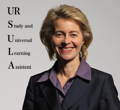
\includegraphics{URSULA.png}

\item \textbf{Who are your prospective users, and how you plan to access them?}\\
The users of the software can be divided into 4 groups: teachers, scientific staff (two different roles), students (inner \& outer), administrative staff.\\
We can access them indirect by email or direct/personal by interviews, meetings or informal conversations.

\item \textbf{What are the users's needs?}\\
The users need an independent plattform that incorporates existing systems and enables them to interact with each other while managing their workflows. The software should create a Blended Learning Environment.
\end{itemize}

\newpage

\textit{Only this page represents the homework.}

\section{Project Brief Introduction}

Today we introduce a completely new and revolutionary Learning Management System (LMS). The first LMS in the world that is not only designed to focus on the users needs but also to support the user's workflow in doing their tasks not just in a very efficent, but also in a very comfortable way. The focus is on a minimalistic concept with eye for the essentials. This revolutionary LMS concentrates on the needs of the members of the following four groups: students, teachers, scientific staff and administrative staff\\
With the upcomming version 2.0 we introduce URSULA, a weak artificial intelligence, that adapts the user's  everyday life by being very flexible, perceptive and customizable. Finally this outstanding software incorporates different systems spreaded over the system scenery of the campus.

\section{Team}

\begin{itemize}
\item \textbf{Tiago Bento}\\
Tiago Bento is a software developer and enthusiast of computer science. He started studying informatics when he was 15 in a technical highschool in Brazil. As he finished highschool, started his computer science graduation in Unicamp among with working in a company where he could learn how to be a professional programmer. Lives in Germany since late 2014 and studies for a year at the Free University of Berlin.
\item \textbf{Nicolas Lehmann}\\
Nicolas Lehmann has a Graduate in Business, a bachelors degree in computer science and studies computer science at the advanced degree level at the Free University of Berlin with the main focus on theoretical computer science, advanced algorithmics and database systems, in particular probabilistic algorithms on Big Data problems. While the previous studies, the minor was consistently psychology and will be the next field of study. Personal interests include general and social psychology and greyhound racing.
\item \textbf{Benjamin Swiers}\\
Benjamin Swiers has an apprenticeship as mathematical-technical software developer, a bachelor's degree in computer science and currently studies computer science at the advanced degree level at the Free University of Berlin. Since 2008 he works for a company that develops software solutions for municipal administrations. In the course of this activity he earned experiences in software development and dealing with customers.
\end{itemize}

\end{document}